\documentclass{lincolncsuthesis}

% Packages you want to use
% Packages you intend to use
% ..

% For example, if you want to render 
% the document in a different font you can
% use something like: 

%\usepackage{gentium}
%\usepackage{txfonts}
%\usepackage[sfdefault]{roboto}


% Or maybe you want clickable references in your thesis:
\usepackage{hyperref}
\usepackage{graphicx}
\usepackage[utf8]{inputenc}
\usepackage[showframe]{geometry}
\usepackage{array, caption, tabularx,  ragged2e,  booktabs}

% Bibliography setup: import bib files
% Add in the .bib files you wish to add 
% into your document here. If you want to
% include others, just copy this line and
% change the path!

\addbibresource{bib/references.bib}


% This thesis template also supports rendering
% a ludography. To cite games, make sure your reference
% in your bib file has keywords={game} in the bibtex item.
%
% See the bib file below for an example.

\addbibresource{bib/ludography.bib}

% Your thesis details -- edit the file at the path below
% so it shows your name, title, etc. 
%% Below are a bunch of details for formatting your undergraduate thesis.
%% Make sure to fill each of these out.

% The title of your thesis (If your title is very large, consider prepending
% it with the \Large command
\title{\bfseries Aerospace Propulsion Laboratory
\newline
\bfseries AE 316}

% Your name, as an author
\author{Spandan Patil}

% The degree
\thesisDegree{}

% The programme
\thesisProgramme{}

% The school name
\thesisSchool{Department of Aerospace Engineering}

% The university you're studying at (Lincoln!)
% The university (UoL)
\thesisUniversity{Indian Institute of Technology, Bombay}

% Your student number
\thesisStudentNumber{180010055}

% The date (which is shown last, you can just put a year in here):
\date{January 2021}



% What will be displayed in the header: the assessment item
\thesisHeaderContents{AE316 180010055}

% Uncommenting the \thesisTurnOffHF line below will remove your name + id from the footer
% as well as removing the header contents. It is NOT recommended to do this
% as the presentation policy for assessed work in the SoCS requires
% these both of these. However, you may want to uncomment this for other
% reasons: i.e. when printing a personal copy which is NOT going to be
% submitted.
% -----
% \thesisTurnOffHF
% -----





\begin{document}

% First, make the title
\maketitle

% Input anything that can go before the acknowledgements 
%% The blank page environment allows you to insert
% pages into your thesis for specific things

\begin{blankpage}
    \chapterTitle{A blank page}
    This is an optional page environment you could use for things like:
	\begin{itemize}
		\item Your own custom preamble chapters (use \texttt{\textbackslash chapterTitle} for titles!)
		\item \emph{``This work is dedicated to...''}
		\item A copyright notice
		\item Additional notes
		\item Quotes
		\item List of publications
		\item An actual blank page
		\item Nomenclature / glossaries, etc.
	\end{itemize}
	It is not recommended to use this in your undergraduate thesis for submission. It has been left in here to make you aware of its existence. This is largely because it does not follow the guidelines set out for undergraduate theses, but you could include this environment for your own personal printed copy. Consult with your supervisor to see if you can use it. 
	
	In addition, you can pass an optional parameter to this environment with the value \texttt{c} to centre this text vertically on the page (use the \texttt{center} environment to align horizontally).
\end{blankpage}

% Then the acknowledgements
%\begin{acknowledgements}
Firstly, I want to thank somebody, and somebody else.\footnote{Here is a footnote} Here is another note.
\end{acknowledgements}

% Then the abstract
%\begin{enumerate}
    \item 'Aircraft Propulsion' by Saeed Farookhi
    \item ‘Fundamental of compressible flows’ by S M Yahya

\end{enumerate}

% Print out the table of tables and table of figures and
% tell the template we're about to start the body of the
% thesis.
\thesisTables
\thesisBodyStart




% start of thesis body
% ---------------------------

% Include introduction
\chapter{Aim}
\begin{enumerate}
    \item 
\end{enumerate}
    \item To see the pressure distribution in Nozzles with various Inlet and Outlet
pressures applied to them.
    \item To identify the type of each nozzle used in the experiment.
\end{itemize}


% Literature review / Background / Related work
\chapter{Setup}
Nozzle Pressure distribution Test Unit will be equipped with the following contents:
\begin{itemize}
    \item 3 Nozzles of unknown configurations with static ports and vanes at
various location to measure pressure at those locations.
    \item Pressure Gauges: Eight pressure Gauges to measure gauge pressure at
several locations.
    \item Rota Meter: Measure air flow range between 1.4 to 9.0gm/s
    \item Fixer: Nozzle is fixed to measure pressure distribution
    \item Input and output Valves
    \item Air Regulator
\end{itemize}

\begin{figure}
    \centering
    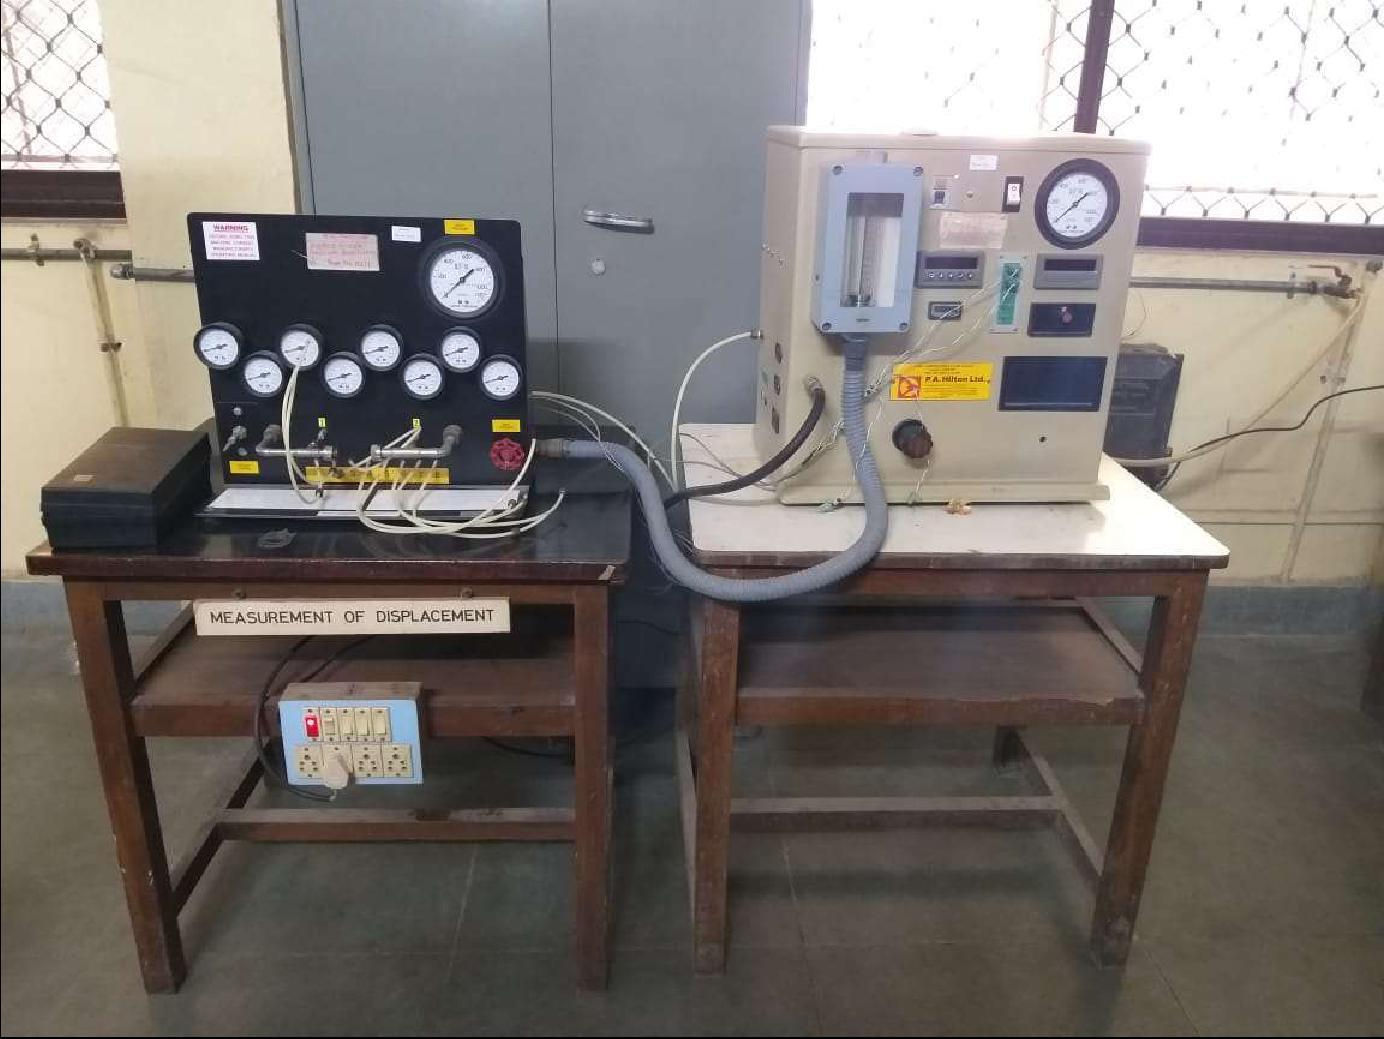
\includegraphics[width=8cm]{setupImg.jpg}
    \caption{Nozzle pressure distribution test unit}
\end{figure}


% Methodology
\chapter{Theory}
{\LARGE Nozzle:}
The basic principal of nozzle is to accelerate the flow along its path. This
can be done with providing a special shape and pressure difference across the
inlet and outlet of the nozzle. For specific type of the flow the shape of nozzle
varies. This variation is as follows:
\begin{figure}[!h]
    \centering
    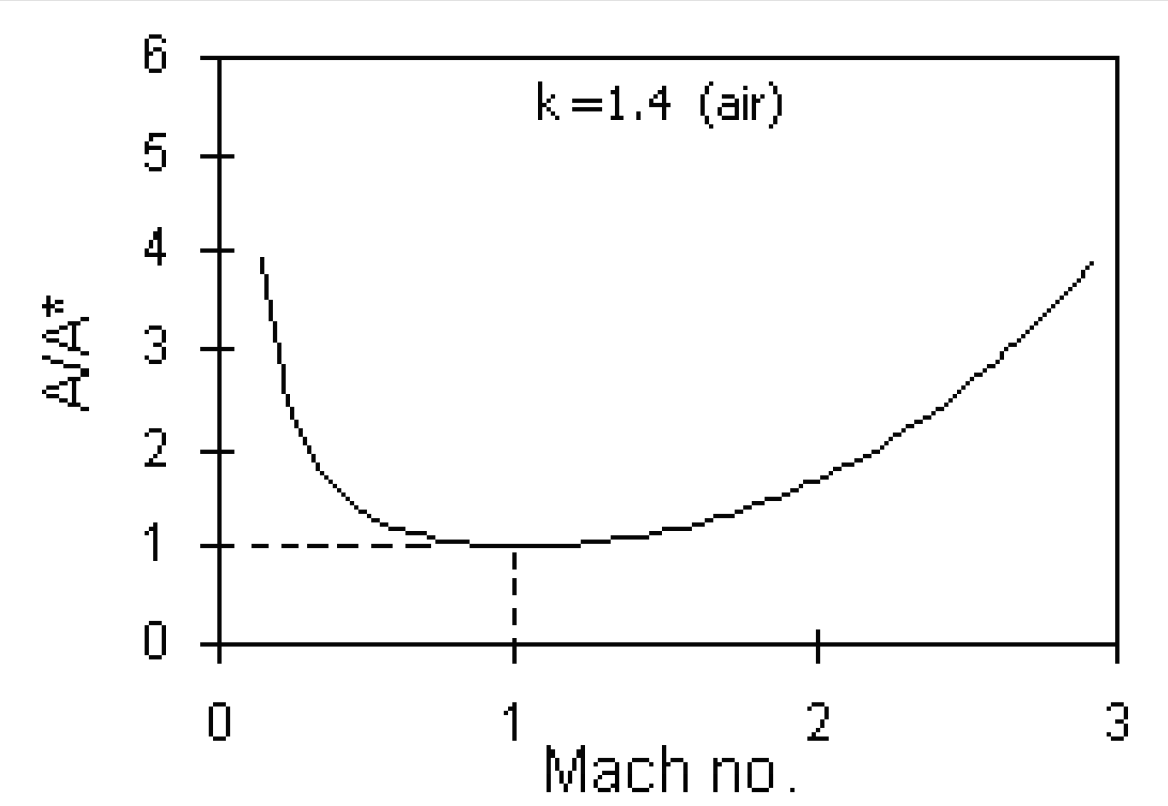
\includegraphics[width=8cm]{areaRatio.png}
    \caption{Area ratio variation with Mach number}
\end{figure}
\newline
Thus, for subsonic flow inlet convergent passage accelerates the flow and for
supersonic flow inlet divergent passage accelerates the flow. As we are going to
encounter flow from static chamber it is necessarily a subsonic flow at inlet.
\newline
Hence we are concerned with following two types of nozzle:
\begin{itemize}
    \item Convergent nozzle
    \item Convergent Divergent nozzle
\end{itemize}
\newpage

{\Large Convergent nozzle:}
This nozzle is mainly used to accelerate the flows till Mach number 1. The pressure distribution along the nozzle for various back pressure values are
shown in following graph.
\begin{figure}[!h]
    \centering
    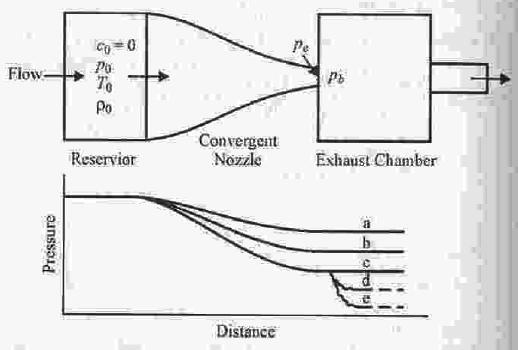
\includegraphics[width=8cm]{convergentNozzle.jpg}
    \caption{Pressure variation across convergent nozzle in Isentropic flow
conditions.}
\end{figure}
\newline
In curve 'a' and 'b', Pb is more than P* and hence, flow is accelerated at less than M=1. Curve 'c' represents design condition where flow is expanded to sonic conditions and Pb=P*. At curve 'c', maximum mass flow condition occurs. For curve 'd' and 'e', Pb<P* and discontinuity in the form of expansion wave occurs at outlet as nozzle can’t accelerate flow to achieve Pb . Thus, nozzle is said chocked at curve 'c' and mass flow rate is constant after that point. The mass flow parameter variation with back pressure variation is as shown below.
\begin{figure}[!h]
    \centering
    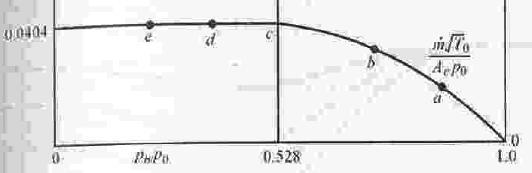
\includegraphics[width=8cm]{convergentMassFlow.jpg}
    \caption{Mass flow parameter variation with pressure ratio}
\end{figure}
\newpage

{\Large Convergent Divergent nozzle:}
This type of nozzle is used to accelerate the subsonic flows to the supersonic
conditions. This contains a convergent section which accelerates the flow to the
sonic condition to throat and a divergent section afterwards which accelerates the sonic flow to the supersonic conditions. Pressure distribution along its path for various back pressure conditions is as shown below.
\begin{figure}[!h]
    \centering
    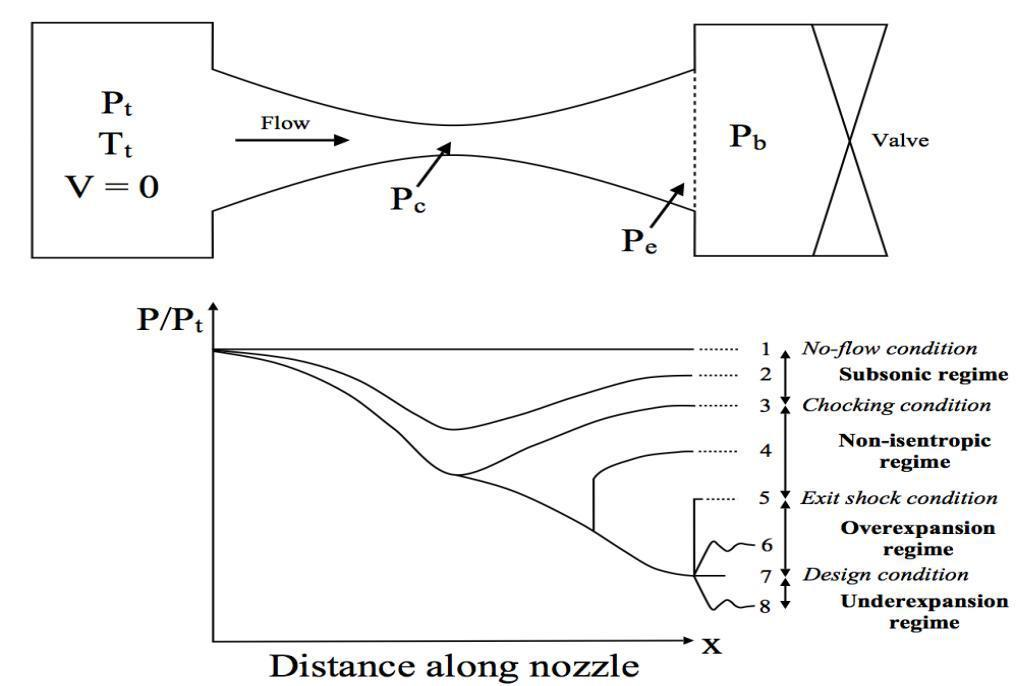
\includegraphics[width=7cm]{CD pressure distribution.jpg}
    \caption{Pressure distribution across CD nozzle}
\end{figure}
\newline
The Mach at throat is less than 1. Here divergent section behaves as diffuser
and increases the flow pressure to achieve Pb. Curve c shows choking condition at
throat i.e. M=1 and divergent section still acts a diffuser.
\newline
Further reducing Pb
means that the divergent section starts acting as nozzle. After some distance a
shock wave appears to increase the pressure and decrease the speed to subsonic.
This discontinuity occurs to match flow pressure to Pb. 
\newline
Curve 7 represents design
condition where expansion occurs in whole nozzle and no discontinuity forms.
This represents the maximum possible isentropic expansion done with nozzle.
\newline
Curve 8 represents the under expansion condition where exit pressure is more
than Pb. Thus, an expansion wave occurs at the exit of the nozzle.
Maximum mass flow parameter occurs at curve 3 and remains constant since. This represents the choking condition.
\newpage
All these mass flow variations can be seen in figure given below.
\begin{figure}[!h]
    \centering
    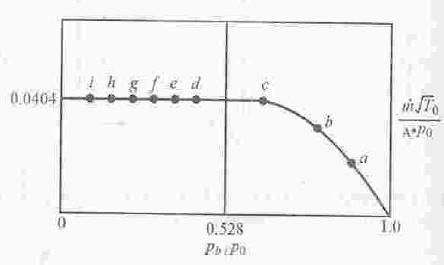
\includegraphics[width=6cm]{CD mass flow.jpg}
    \caption{Variation of mass flow parameter with pressure ratio}
\end{figure}


\chapter{Experimental Details}
We will be looking at all the details and procedure of our analysis.

\section{Procedure}
\begin{enumerate}
    \item Start the testing apparatus by making necessary arrangements like checking pressure valve and see if inlet pressure is sufficient enough.
    \item Mount the nozzle whose pressure distribution is to be measured and
connect pressure pipes with vanes of Nozzle.
    \item First keep the inlet gauge pressure as 500 kN/m2 constant and take
reading of all pressures across nozzle by varying the exit pressure from 0 to
400 KN/m2.
    \item Then keep exit pressure as 50kN/m2 constant and take reading of all
pressures across nozzle by varying the inlet pressure.
    \item Tabulate the readings and do necessary calculations.
    \item Plot relevant graphs as mentioned.
    \item Repeat the procedures 2-6 for different nozzles given.
\end{enumerate}

\newpage
\section{Block diagram of experimental Set-up}
\begin{figure}[!h]
    \centering
    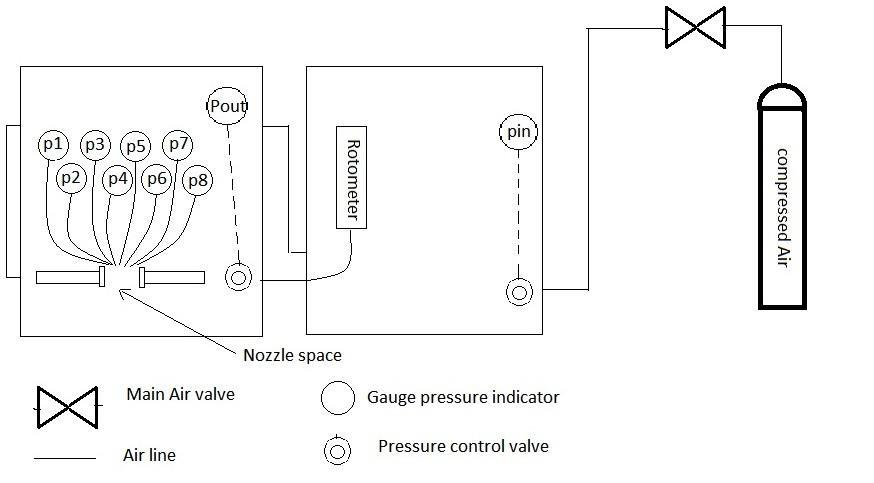
\includegraphics[width=16cm]{experimental setup.jpg}
    \caption{Experimental Setup}
\end{figure}


\section{Observation}
\[Ambient pressure = 101.325kN/m^2\]
\begin{itemize}
    \item {\Large Nozzle A}
        
{\tiny
\noindent\setlength\tabcolsep{4pt}%
\begin{tabularx}{\linewidth}{|c|c|*{10}{>{\RaggedRight\arraybackslash}X|}}
  \hline
   Pi kN/m2 & Po kN/m2 & Pressure ratio & Mass flow rate (g/s) & p1 kN/m2 & p2 kN/m2 & p3 kN/m2 & p4 kN/m2 & p5 kN/m2 & p6 kN/m2 & p7 kN/m2 & p8 kN/m2   \\
  \hline
  601.325 & 151.325 & 0.25165 & 4.4 & 541.325 & 321.325 & 221.325 & 151.325	& 111.325 & 91.325	& 101.325	& 101.325 \\
  \hline
  601.325	& 201.325	& 0.33480	& 4.4	& 541.325	& 321.325	& 221.325	& 151.325	& 111.325	& 91.325	& 101.325	& 181.325 \\
  \hline
  601.325	& 251.325	& 0.41795	& 4.4	& 541.325	& 321.325	& 221.325	& 151.325	& 111.325	& 101.325	& 221.325	& 231.325 \\
  \hline
  601.325	& 301.325	& 0.50110	& 4.4	& 541.325	& 321.325	& 221.325	& 181.325	& 241.325	& 251.325	& 281.325	& 181.325 \\
  \hline
  601.325	& 351.325	& 0.58425	& 4.4	& 541.325	& 321.325	& 221.325	& 271.325	& 281.325	& 301.325	& 331.325	& 341.325 \\
  \hline
  601.325	& 401.325	& 0.66740	& 4.4	& 541.325	& 321.325	& 231.325	& 321.325	& 331.325	& 351.325	& 381.325	& 401.325 \\
  \hline
\end{tabularx}
\captionof{table}{Constant Inlet Pressure 601.325 kN/m2}}
\vskip1cm

{\tiny
\noindent\setlength\tabcolsep{4pt}%
\begin{tabularx}{\linewidth}{|c|c|*{10}{>{\RaggedRight\arraybackslash}X|}}
  \hline
   Pi kN/m2 & Po kN/m2 & Pressure ratio & Mass flow rate (g/s) & p1 kN/m2 & p2 kN/m2 & p3 kN/m2 & p4 kN/m2 & p5 kN/m2 & p6 kN/m2 & p7 kN/m2 & p8 kN/m2   \\
  \hline
  251.325	& 151.325	& 0.60211	& 1.6	& 231.325	& 141.325	& 101.325	& 111.325	& 121.325	& 131.325	& 141.325	& 151.325 \\
  \hline
  301.325	& 151.325	& 0.50220	& 2	& 271.325	& 271.325	& 111.325 & 101.325	& 111.325	& 121.325	& 141.325	& 151.325 \\
  \hline
  351.325	& 151.325	& 0.43073	& 2.4	& 321.325	& 181.325	& 131.325	& 101.325	& 101.325	& 121.325	& 141.325	& 141.325 \\
  \hline
  401.325	& 151.325	& 0.37706	& 2.8	& 361.325	& 221.325	& 141.325	& 101.325	& 81.325	& 91.325	& 111.325	& 141.325 \\
  \hline
  451.325	& 151.325	& 0.33529	& 3.2	& 401.325	& 241.325	& 161.325	& 111.325	& 81.325	& 71.325	& 111.325	& 131.325 \\
  \hline
  501.325	& 151.325	& 0.30185	& 3.6	& 451.325	& 261.325	& 181.325	& 121.325	& 91.325	& 71.325	& 81.325	& 131.325 \\
  \hline
  551.325	& 151.325	& 0.27447	& 4	& 491.325	& 291.325	& 201.325	& 131.325	& 101.325	& 81.325	& 91.325	& 111.325 \\
  \hline
  601.325	& 151.325	& 0.25165	& 4.4	& 541.325	& 321.325	& 221.325	& 151.325	& 111.325	& 91.325	& 101.325	& 101.325 \\
  \hline
\end{tabularx}
\captionof{table}{Constant Outlet Pressure 151.325 kN/m2}}
\vskip1cm

    \item {\Large Nozzle B}

{\tiny
\noindent\setlength\tabcolsep{4pt}%
\begin{tabularx}{\linewidth}{|c|c|*{7}{>{\RaggedRight\arraybackslash}X|}}
  \hline
   Pi kN/m2 & Po kN/m2 & Pressure ratio & Mass Flow Rate (g/s) & p1 kN/m2 & p2 kN/m2 & p3 kN/m2 & p4 kN/m2 & p5 kN/m2  \\
  \hline
  601.325	& 151.325	& 0.25165	& 4.4	& 521.325	& 281.325	& 221.325	& 181.325	& 121.325 \\
  \hline
  601.325	& 201.325	& 0.33480	& 4.4	& 531.325	& 281.325	& 211.325	& 181.325	& 141.325 \\
  \hline
  601.325	& 251.325	& 0.41795	& 4.4	& 531.325	& 281.325	& 211.325	& 181.325	& 201.325 \\
  \hline
  601.325	& 301.325	& 0.50110	& 4.4	& 531.325	& 281.325	& 211.325	& 181.325	& 271.325 \\
  \hline
  601.325	& 351.325	& 0.58425	& 4.4	& 531.325	& 281.325	& 211.325	& 301.325	& 331.325 \\
  \hline
  601.325	& 401.325	& 0.66740	& 4.4	& 531.325	& 281.325	& 271.325	& 361.325	& 381.325 \\
  \hline
\end{tabularx}
\captionof{table}{Constant Inlet Pressure 601.325 kN/m2}}
\vskip1cm


{\tiny
\noindent\setlength\tabcolsep{4pt}%
\begin{tabularx}{\linewidth}{|c|c|*{7}{>{\RaggedRight\arraybackslash}X|}}
  \hline
   Pi kN/m2 & Po kN/m2 & Pressure ratio & Mass Flow Rate (g/s) & p1 kN/m2 & p2 kN/m2 & p3 kN/m2 & p4 kN/m2 & p5 kN/m2  \\
  \hline
  251.325	& 151.325	& 0.60211	& 1.6	& 221.325	& 121.325	& 111.325	& 121.325	& 141.325 \\
  \hline
  301.325	& 151.325	& 0.50219	& 2	& 261.325	& 141.325	& 111.325	& 121.325	& 121.325 \\
  \hline
  351.325	& 151.325	& 0.43073	& 2.4	& 311.325	& 161.325	& 121.325	& 101.325	& 111.325 \\
  \hline
  401.325	& 151.325	& 0.37706	& 2.8	& 351.325	& 186.325	& 141.325	& 111.325	& 101.325 \\
  \hline
  451.325	& 151.325	& 0.33529	& 3.2	& 391.325	& 201.325	& 161.325	& 131.325	& 101.325 \\
  \hline
  501.325	& 151.325	& 0.30185	& 3.6	& 441.325	& 231.325	& 181.325	& 151.325	& 111.325 \\
  \hline
  551.325	& 151.325	& 0.27447	& 4	& 481.325	& 261.325	& 201.325	& 161.325	& 121.325 \\
  \hline
  601.325	& 151.325	& 0.25165	& 4.4	& 521.325	& 281.325	& 221.325	& 181.325	& 121.325 \\
  \hline
\end{tabularx}
\captionof{table}{Constant Outlet Pressure 151.325 kN/m2}}
\vskip1cm
\newpage

    \item {\Large Nozzle C}
    
{\tiny
\noindent\setlength\tabcolsep{4pt}%
\begin{tabularx}{\linewidth}{|c|c|*{8}{>{\RaggedRight\arraybackslash}X|}}
  \hline
   Pi kN/m2 & Po kN/m2 & Pressure ratio & Mass Flow Rate (g/s) & p1 kN/m2 & p2 kN/m2 & p3 kN/m2 & p4 kN/m2 & p5 kN/m2 & p6 kN/m2  \\
  \hline
  601.325	& 151.325	& 0.25165	& 4.2	& 561.325	& 551.325	& 531.325	& 471.325	& 351.325	& 341.325 \\
  \hline
  601.325	& 201.325	& 0.33480	& 4.2	& 561.325	& 551.325	& 531.325	& 471.325	& 361.325	& 341.325 \\
  \hline
  601.325	& 251.325	& 0.41795	& 4.2	& 561.325	& 551.325	& 531.325	& 471.325	& 351.325	& 341.325 \\
  \hline
  601.325	& 301.325	& 0.50110	& 4.2	& 561.325	& 551.325	& 531.325	& 471.325	& 351.325	& 341.325 \\
  \hline
  601.325	& 351.325	& 0.58425	& 4.2	& 561.325	& 551.325	& 531.325	& 471.325	& 361.325	& 351.325 \\
  \hline
  601.325	& 401.325	& 0.66740	& 4.2	& 571.325	& 561.325	& 541.325	& 481.325	& 401.325	& 391.325 \\
  \hline
\end{tabularx}
\captionof{table}{Constant Inlet Pressure 601.325 kN/m2}}
\vskip1cm

{\tiny
\noindent\setlength\tabcolsep{4pt}%
\begin{tabularx}{\linewidth}{|c|c|*{8}{>{\RaggedRight\arraybackslash}X|}}
  \hline
   Pi kN/m2 & Po kN/m2 & Pressure ratio & Mass Flow Rate (g/s) & p1 kN/m2 & p2 kN/m2 & p3 kN/m2 & p4 kN/m2 & p5 kN/m2 & p6 kN/m2  \\
  \hline
  251.325	& 151.325	& 0.60211	& 1.5	& 241.325	& 241.325	& 231.325	& 201.325	& 151.325	& 151.325 \\
  \hline
  301.325	& 151.325	& 0.50219	& 2	& 291.325	& 281.325	& 271.325	& 241.325	& 181.325	& 161.325 \\
  \hline
  351.325	& 151.325	& 0.43072	& 2.4	& 331.325	& 331.325	& 321.325	& 281.325	& 211.325	& 181.325 \\
  \hline
  401.325	& 151.325	& 0.37706	& 2.8	& 381.325	& 371.325	& 361.325	& 321.325	& 241.325	& 221.325 \\
  \hline
  451.325	& 151.325	& 0.33529	& 3.1	& 431.325	& 421.325	& 401.325	& 361.325	& 271.325	& 251.325 \\
  \hline
  501.325	& 151.325	& 0.30185	& 3.4	& 471.325	& 461.325	& 451.325	& 391.325	& 301.325	& 281.325 \\
  \hline
  551.325	& 151.325	& 0.27447	& 3.8	& 521.325	& 511.325	& 491.325	& 431.325	& 431.325	& 301.325 \\
  \hline
  601.325	& 151.325	& 0.25165	& 4.2	& 561.325	& 551.325	& 531.325	& 471.325	& 351.325	& 341.325 \\
  \hline
\end{tabularx}
\captionof{table}{Constant Outlet Pressure 151.325 kN/m2}}
\vskip1cm

\end{itemize}

\section{Plots}
Here are the plots obtained from Observation Tables. We will be using python for accurate plots. All the plots show pressure ratios at different locations of Nozzle.
\newline
Here is a snippet of Python code used for one of the plots:

\begin{framed}
\begin{minted}[breaklines]{python}
import numpy as np
import matplotlib.pyplot as plt
from scipy import interpolate
a=['541.325 321.325 221.325 151.325 111.325 91.325 101.325 101.325',
'541.325 321.325 221.325 151.325 111.325 91.325 101.325 181.325',
'541.325 321.325 221.325 151.325 111.325 101.325 221.325 231.325',
'541.325 321.325 221.325 181.325 241.325 251.325 281.325 181.325',
'541.325 321.325 221.325 271.325 281.325 301.325 331.325 341.325',
'541.325 321.325 231.325 321.325 331.325 351.325 381.325 401.325']
b=[601.325,601.325,601.325,601.325,601.325,601.325]
c=[151.325,201.325,251.325,301.325,351.325,401.325]
net=[]
for i in a:
    k = i.split()
    net.append([float(j) for j in k])

x_scatter = np.array([i for i in range(len(net[0])+1)][1:])
x=np.linspace(x_scatter[0], x_scatter[-1], 300)
for i in range(len(a)):
    y = np.array([j/b[i] for j in net[i]])
    plt.scatter(x_scatter, y, s=10)
    y_2 = interpolate.make_interp_spline(x_scatter, y)
    y_new = y_2(x)
    plt.plot(x, y_new)

legend1=[]
for i in range(len(a)):    
    legend1.append('Poutlet='+str(c[i])+'kN/m2')
    
plt.legend(legend1, loc='best', prop={'size': 8})   
plt.xlabel('Locations')
plt.ylabel('Pressure Ratio')
plt.show()
\end{minted}
\end{framed}

\newpage
\begin{itemize}
    \item \centering {\large Nozzle A: Constant Inlet Pressure 601.325 kN/m2}
    
    \begin{figure}[!h]
    \centering
    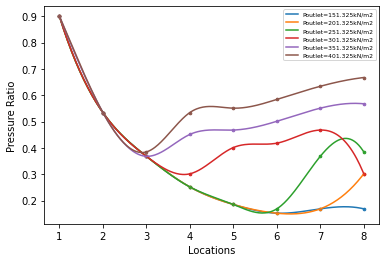
\includegraphics[width=12cm]{figure 1.png}
    \caption{Nozzle A Constant Inlet Pressure Plot}
\end{figure}

    \item \centering {\large Nozzle A: Constant Outlet Pressure 151.325 kN/m2}
     \begin{figure}[!h]
    \centering
    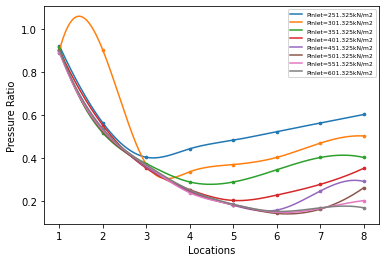
\includegraphics[width=12cm]{figure 2.png}
    \caption{Nozzle A Constant Outlet Pressure Plot}
\end{figure}
\newline
{\tiny Note: Ignore the spike between p1 and p2 at Pinlet=201.325kN/m2 as it was interpreted by spline python for getting an approximate function}

    \item \centering {\large Nozzle B: Constant Inlet Pressure 601.325 kN/m2}
    \begin{figure}[!h]
    \centering
    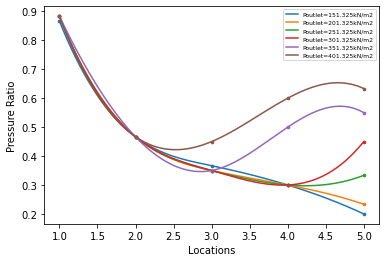
\includegraphics[width=12cm]{figure 3.png}
    \caption{Nozzle B Constant Inlet Pressure Plot}
\end{figure}

    \item \centering {\large Nozzle B: Constant Outlet Pressure 151.325 kN/m2}
    \begin{figure}[!h]
    \centering
    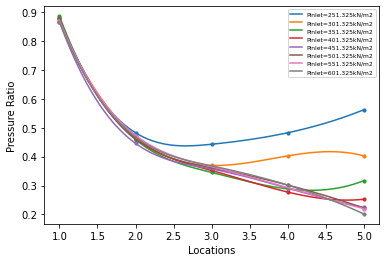
\includegraphics[width=12cm]{figure 4.png}
    \caption{Nozzle B Constant Outlet Pressure Plot}
\end{figure}

\newpage
    \item \centering {\large Nozzle C: Constant Inlet Pressure 601.325 kN/m2}
    \begin{figure}[!h]
    \centering
    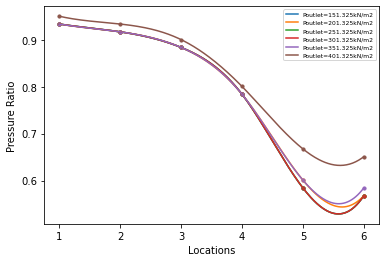
\includegraphics[width=12cm]{figure 5.png}
    \caption{Nozzle C Constant Inlet Pressure Plot}
\end{figure}


    \item \centering {\large Nozzle C: Constant Outlet Pressure 151.325 kN/m2}
    \begin{figure}[!h]
    \centering
    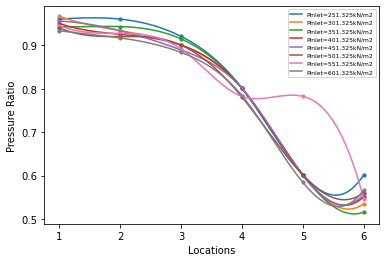
\includegraphics[width=12cm]{figure 6.png}
    \caption{Nozzle C Constant Outlet Pressure Plot}
\end{figure}
\end{itemize}
\newpage

We also need to plot Mass flow Rate wrt to pressure ratios. Snippet of the python code is as follows:
\begin{framed}
\begin{minted}[breaklines]{python}
import numpy as np
import matplotlib.pyplot as plt
from scipy import interpolate

mfr1 =np.array([4.4,4.4,4.4,4.4,4.4,4.4])
pr1=np.array([0.2516526005,0.3348023116,0.4179520226,0.5011017337,
0.5842514447,0.6674011558])
plt.scatter(pr1, mfr1)
x=np.linspace(pr1[0], pr1[-1],300)
k = interpolate.make_interp_spline(pr1, mfr1)
y_new = k(x)
plt.plot(x, y_new)

\end{minted}
\end{framed}

\begin{itemize}
    \item \centering {\large Constant Inlet Pressure 601.325 kN/m2}
    \begin{figure}[!h]
    \centering
    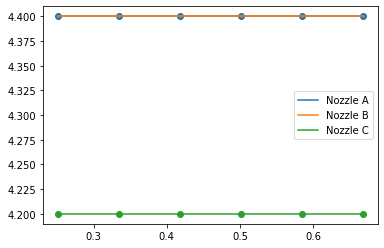
\includegraphics[width=12cm]{figure 7.png}
    \caption{Mass Flow Rate(y-axis) vs Pressure Ratio Plot(x-axis)}
\end{figure}

    \item \centering {\large Constant Outlet Pressure 151.325 kN/m2}
    \begin{figure}[!h]
    \centering
    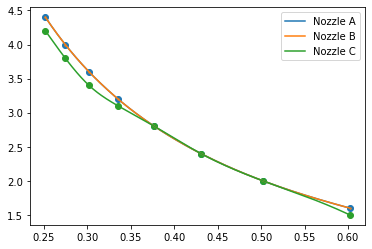
\includegraphics[width=12cm]{figure 8.png}
    \caption{Mass Flow Rate(y-axis) vs Pressure Ratio Plot(x-axis)}
\end{figure}
\end{itemize}




    


\chapter{Conclusions}
\begin{enumerate}
    \item Nozzle A shows decrease and further increase in pressure across the locations. Hence, we can conclude it as a CD Nozzle.
    \item Throat of Nozzle A seems to be near location 3 as pressure decreases till that location and then starts rising for higher Pressure Ratios.
    
    \item TO write
    \item Nozzle B shows decrease and further increase in pressure across locations. Hence, it is a CD Nozzle.
    \item Throat of Nozzle B seems to be near location 2 as pressure decreases till that point and increases further.
    \item Design Pressure Ratio of Nozzle B is around 0.3 since the pressure graph goes horizontal.
    \item Nozzle C shows decrease in pressure ratios over locations indicating a convergent Nozzle.
    
\end{enumerate}

\chapter{References}
\begin{enumerate}
    \item 'Aircraft Propulsion' by Saeed Farookhi
    \item ‘Fundamental of compressible flows’ by S M Yahya

\end{enumerate}






% end of thesis body
% --------------------------

% Print out the references
\printReferences

% Print out the ludography (optional -- you can comment this out if you're not gonna cite games)
\printLudography

% If you want to put some text before the list of games,
% then you can use the following code:
%\begin{ludography}[Ludography / Optional Title]
    %Here are some games.
%\end{ludography}


% Appendices: feel free to comment these out if you are 
% not going to use them.
%\include{chapters/appendices}


\end{document}
